\documentclass{article}


\usepackage[russian]{babel}
\usepackage{mathtext, amsmath, caption, geometry, amssymb, graphicx, wrapfig}
\captionsetup[table]{position=t,justification=raggedleft,slc=off}
%\setlength{\abovecaptionskip}{0pt}
\geometry{left=3cm, right=1.5cm, top=2cm, bottom=2cm}

\newcommand{\w}{\vec}

\title{Лабораторная работа №3.4.1. \\ \textbf{Измерение магнитной восприимчивости диа- и парамагнетиков}}
\author{Михаил Орлов, Павел Рудачихин, Б04-507}
\date{01.09.2026}

\begin {document}

\maketitle{}

\section {Аннотация} 

	\hspace{4mm} Цель работы -- измерение магнитной восприимчивости образцов меди, графита и алюминия методом Гюи.
	

\section {Теоретическое введение}

	\subsection{Магнитное поле в веществе. Диа- и парамагнетики}

		\hspace{4mm} Для макроскопического описания магнитных свойств среды используется вектор намагниченности $\w{M}$ -- магнитный момент единичного объёма вещества. 
		
		Введя вспомогательный вектор напряжённости магнитного поля $\w{H}$, можно расписать результирующее магнитное поле (индукцию поля) $\w{B}$:
		
		\begin{equation}
			\w{B} = \mu_0(\w{H} + \w{M}),
		\end{equation}
		
		где $\mu_0$ -- магнитная постоянная.
	
		В простейшем случае имеет место связь
		
		\begin{equation}
			\w{M} = \chi \w{H}
		\end{equation}
		
		где $\chi$ -- магнитная восприимчивость. Вещества, для которых выполняется закон (2) называют парамагнетиками, если $\chi > 0$, и диамагнетиками иначе.
		
		
		
		
	\subsection{Метод Гюи измерения магнитной восприимчивости}
	
	\hspace{4mm} В методе Гюи используется образец в виде тонкого длинного стержня, один из концов которого помещают в однородное поле (в зазор электромагнита), а другой -- в область, где полем можно пренебречь (вне зазора). 
	
	Если площадь сечения образца равна $S$, его магнитная восприимчивость -- $\chi$, поле в зазоре -- $B_0$, то сила, действующая на образец, равна
	
	\begin{equation}
		F \approx \chi \frac{B_0^2}{2\mu_0}S
	\end{equation}
	
	Следовательно, парамагнетики втягиваются в зазор электромагнита, а диамагнетики -- выталкиваются.
	
	
\section{Описание установки}
	
	\begin{wrapfigure}{r}{0.5\linewidth}
		\centering
		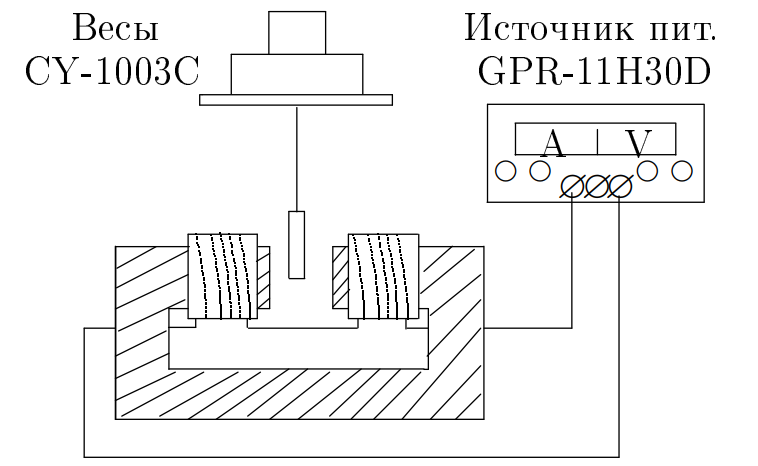
\includegraphics[width=\linewidth]{setup}
		\caption{Схема установки}
		\label{fig:2}
	\end{wrapfigure}
	\hspace{4mm} Схема установки приведена на рисунке 1. В зазоре электромагнита создаётся постоянное магнитное поле, достаточно однородное в средней части зазора из-за большого диаметра полюсов по сравнению с шириной зазора. Обмотки электромагнита подключены к источнику питания GPR-11H30D. 
	
	Данный источник питания использовался в режиме постоянного тока (CC). Изменение индукции магнитного поля происходило путём изменения тока в обмотках. Градуировка электромагнита (зависимость магнитного поля от тока в обмотках $B(I)$) выполнялась с помощью милливеберметра  по формуле 
	
	\begin{equation}
		B = \frac{\Delta\Phi}{SN}
	\end{equation}
	
	где $\Delta\Phi$ - показания милливеберметра (изменение потока магнитной индукции), $SN$ -- площадь и число витков катушки милливеберметра ($SN = 72$ см$^2$).
	
	Образцы подвешиваются к весам CY-1003C, по которым определяется перегрузка -- сила, действующая со стороны магнитного поля на образец.
	
	
\section{Результаты и обсуждения}

	\subsection{Градуировка электромагнита}
	
		Зависимость $\Delta\Phi(I)$ снята в интервале токов до 3А. По формуле 4 получена зависимость $B(I)$ и построен соответствующий график (см. рис. 2). Точки с хорошей точностью ложатся на прямую $B = kI$, где $k = (0,282 \pm 0,006) $ Тл/А определён по методу наименьших квадратов. Следовательно, сердечник не входит в насыщение (для электротехнической стали 1,5 -- 2 Тл, тогда как в работе максимальная индукции 0,9 Тл).
		
		\begin{figure}[h!]
			\centering
			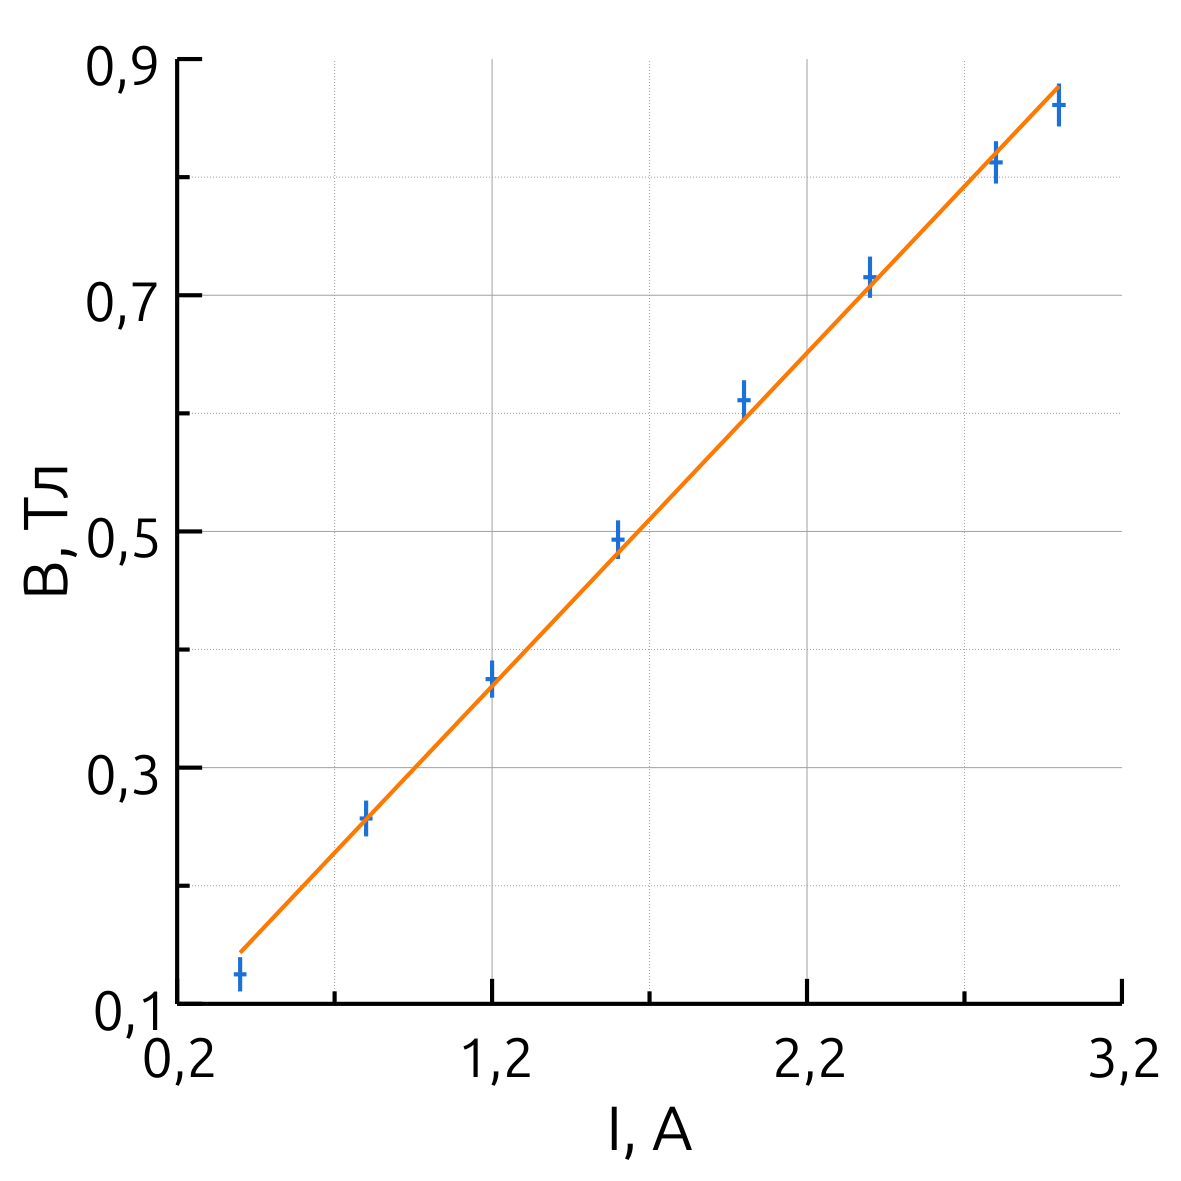
\includegraphics[width=0.7\linewidth]{BI}
			\caption{Градуировка электромагнита $B(I)$}
			\label{fig:1}
		\end{figure}
	
	\subsection{Основная серия эксперимента}
	
	Зависимость перегрузки образца от тока через электромагнит $F(I)$ снята на увеличении и уменьшении тока. Расхождение на прямом и обратном ходе не превышает погрешности измерения перегрузки, поэтому график построен по средним арифметическим соответствующих перегрузок. По полученной ранее градуировке переходим от зависимости $F(I)$ к $F(B)$, строим график в координатах $|F|(B^2)$ (см. рис. 3). Прямые для меди и алюминия построены в одних координатах. 
	
	
	
	\begin{figure}[h!]
		\centering
		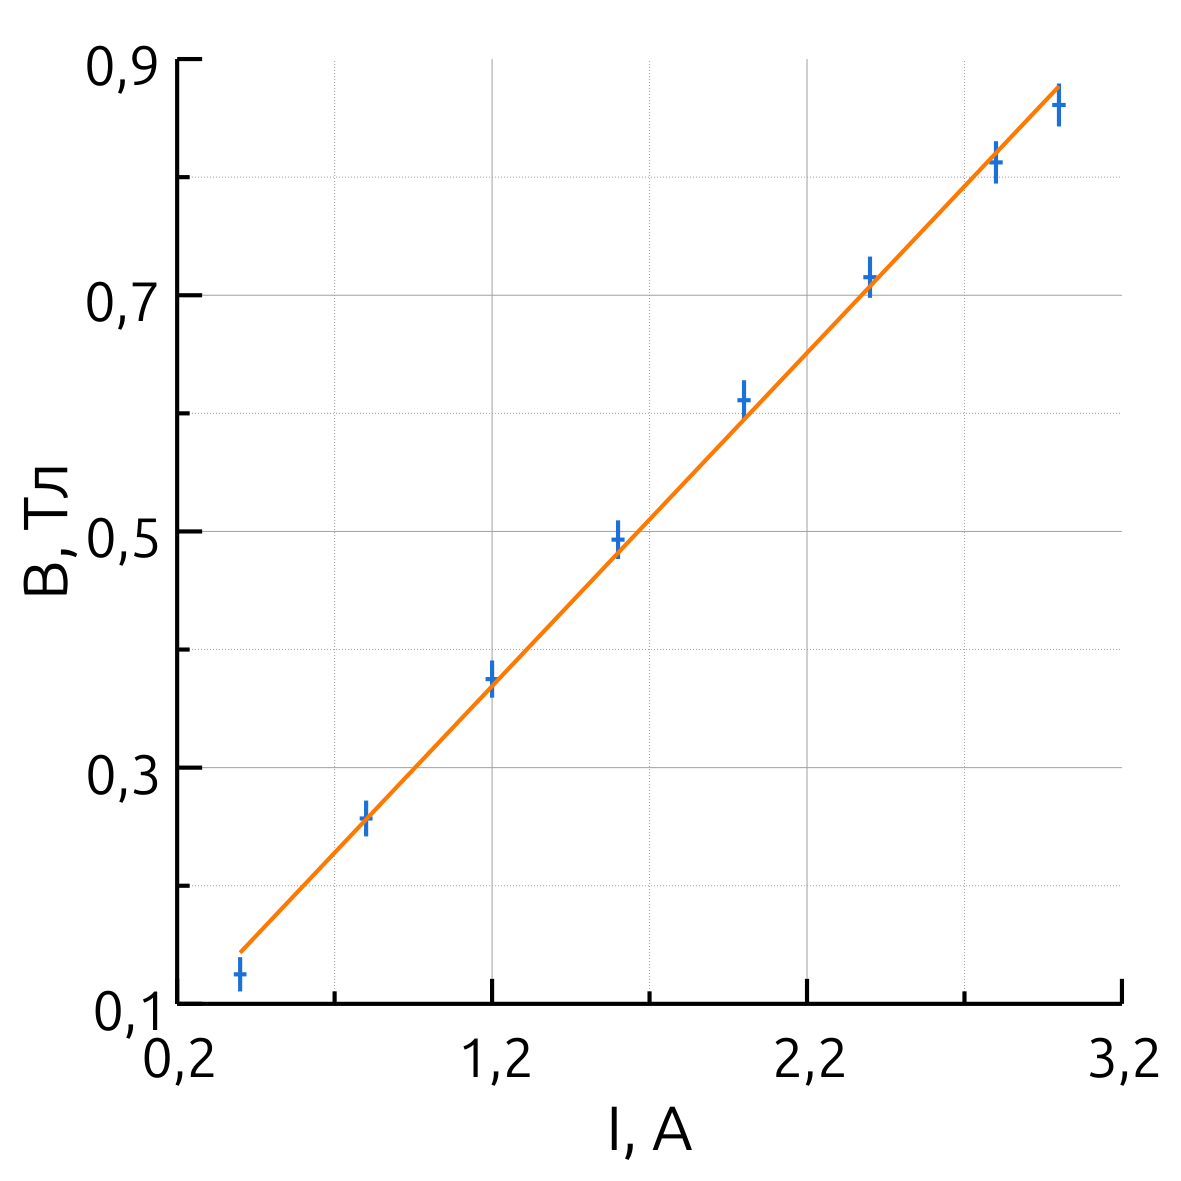
\includegraphics[width=0.7\linewidth]{BI}
		\caption{Градуировка электромагнита $B(I)$}
		\label{fig:}
	\end{figure}
	
	
	

	

\section{Выводы}



\section{Приложение}

	\subsection{Параметры образцов}
	
	\begin{table}[h!]
		\centering
		\begin{tabular}{|c|c|c|c|}
			\hline
			Образец & Al & Cu & C \\
			\hline
			m, г & 26,00 & 84,00 & 3,67 \\
			\hline
			d, см & 1,0 & 1,0 & 0,5 \\
			\hline
		\end{tabular}
	\end{table}

	\subsection{Градуировка электромагнита}
	
	\begin{table}[h!]
		\centering
		\begin{tabular}{|c|c|c|c|c|c|c|c|c|}
			\hline
			$I$, А & 0,4 & 0,8 & 1,2 & 1,6 & 2,0 & 2,4 & 2,8 & 3,0 \\
			\hline
			$\Phi$, мВб & 0,90 & 1,85 & 2,70 & 3,55 & 4,40 & 5,15 & 5,85 & 6,20 \\
			\hline
		\end{tabular}
	\end{table}

\end {document}